\newsection
\section{Технический проект}
\subsection{Общие сведения о программной системе}

Необходимо спроектировать и разработать программную систему учёта для создания услуг технического обслуживания сельскохозяйственной техники.

Разрабатываемая программная система учёиа (ПСУ) предназначена для автоматизации и упрощении процессов учёта и управления данными, что позволяет эффективно управлять ресурсами, контролировать финансовые операции и принимать обоснованные управленческие решения.

Основной принцип работы программной системы учёта заключается в автоматизации и систематизации процессов учёта и управления данными в организации. Вот основные этапы и принципы работы такой системы:
\begin{enumerate}
	\item Сбор данных:
	Первый этап работы программной системы учёта состоит в сборе данных из различных источников, таких как финансовые транзакции, данные о клиентах, информация о запасах и т.д. Эти данные могут поступать из внутренних и внешних источников, включая бухгалтерскую отчётность, платёжные системы, CRM-системы и другие.
	\item Хранение данных:
	После сбора данные сохраняются в централизованной базе данных или в нескольких связанных базах данных. Это обеспечивает целостность, доступность и безопасность данных, а также обеспечивает возможность их последующей обработки и анализа.
	\item Обработка данных:
	Программная система учёта обрабатывает собранные данные согласно определённым алгоритмам и правилам. Это включает в себя проведение бухгалтерских операций, расчёты финансовых показателей, анализ клиентской активности и многое другое. Обработка данных может быть автоматизирована с использованием специализированных алгоритмов и инструментов.
	\item Анализ и отчётность:
	После обработки данные анализируются с целью выявления тенденций, определения ключевых показателей эффективности и принятия управленческих решений. Программная система учёта предоставляет различные инструменты для генерации отчётов, дашбордов и аналитических данных, которые помогают руководству принимать информированные решения.
	\item Управление и контроль:
	Программная система учёта также обеспечивает возможность управления и контроля за финансами, запасами, клиентскими отношениями и другими аспектами бизнеса. Это включает в себя установление бюджетов, контроль выполнения планов, мониторинг финансовых показателей и принятие корректирующих мер при необходимости.
\end{enumerate}

Принцип работы программной системы учёта основан на автоматизации и систематизации бизнес-процессов, что позволяет организации эффективно управлять ресурсами, контролировать финансовые операции и принимать обоснованные управленческие решения.


\subsection{Проектирование архитектуры программной системы}
\subsubsection{Выбор архитектурного стиля и паттернов проектирования}
Для разработки программной системы учёта могут быть использованы различные паттерны проектирования в зависимости от требований проекта и архитектурных особенностей. Однако, одним из наиболее подходящих паттернов может быть Model-View-Controller (MVC).

Паттерн MVC предоставляет чёткое разделение бизнес-логики приложения (Модель), пользовательского интерфейса (Представление) и механизмов управления пользовательским вводом (Контроллер). Вот как этот паттерн может быть применён к программной системе учёта:

Преимущества применения паттерна MVC в разработке программной системы учёта включают чёткое разделение ответственностей между компонентами, повышение переиспользуемости кода, облегчение тестирования и поддержки системы. Кроме того, этот паттерн обеспечивает гибкость и расширяемость системы, что позволяет легко вносить изменения и добавлять новую функциональность по мере необходимости.

\subsubsection{Структура базы данных}

Структура базы данных программной системы учёта может значительно различаться в зависимости от конкретных требований и функциональности системы. Однако, в качестве примера, я могу предложить базовую структуру для системы учёта, которая включает основные сущности и их взаимосвязи:

\begin{enumerate}
	\item Таблица "Пользователи".
	Содержит реквизиты:
	\begin{itemize}
		\item Уникальный идентификатор пользователя;
		\item Имя пользователя;
		\item Хэш пароля пользователя;
		\item Адрес электронной почты пользователя;
		\item Роль пользователя в системе (администратор, менеджер, обычный пользователь и т.д.);
	\end{itemize}
	
	\item Справочник "Контрагенты".
	Содержит реквизиты: 
	\begin{itemize}
		\item Уникальный идентификатор контрагента;
		\item ФИО контрагента;
		\item Адрес электронной почты контрагента;
		\item Номер телефона контрагента;
		\item Адрес контрагента;
	\end{itemize}
	
	\item Справочник "Запчасти".
	Содержит реквизиты: 
	\begin{itemize}
		\item Серийный номер запчасти;
		\item Наименование;
		\item Для какой техники предназначена запчасть;
	\end{itemize}
	
	\item Справочник "Техника".
	Содержит реквизиты: 
	\begin{itemize}
		\item Серийный номер техники;
		\item Наименование;
	\end{itemize}
\end{enumerate}

\subsubsection{Описание паттерна}

Программная система будет включать в себя следующий паттерн:

\begin{itemize}
	\item Модель (Model): В этой части системы располагается бизнес-логика, отвечающая за управление данными и бизнес-правилами. Модель включает в себя классы и компоненты, отвечающие за учёт финансовых операций, управление запасами, учёт клиентов и другие аспекты функциональности системы.
	\item Представление (View): Эта часть системы отвечает за отображение данных и интерактивное взаимодействие с пользователем. Представление может быть реализовано в виде веб-интерфейса, мобильного приложения или других клиентских приложений. Оно предоставляет пользователю удобный доступ к функциональности системы и позволяет визуализировать данные в удобном формате.
	\item Контроллер (Controller): Контроллеры являются посредниками между пользовательским интерфейсом и бизнес-логикой. Они обрабатывают пользовательский ввод, вызывают соответствующие методы модели для обработки запросов и обновления данных, а затем обновляют представление с учётом результатов.
\end{itemize}


\subsubsection{Планирование докеризации и оркестрации сервисов}

Для планирования докеризации и оркестрации сервисов программной системы учёта, мы можем разделить процесс на несколько этапов:

\begin{enumerate}
	\item Идентификация сервисов:Определите все компоненты системы, которые будут докеризованы. Это может включать базу данных, веб-сервер, бэкенд-сервисы, фронтенд-приложения и т.д; 
	\item Определите все компоненты системы, которые будут докеризованы. Это может включать базу данных, веб-сервер, бэкенд-сервисы, фронтенд-приложения и т.д.;
	\item Создание Dockerfile: Для каждого сервиса создайте Dockerfile, описывающий, как собрать образ контейнера. В Dockerfile должны быть указаны все зависимости, настройки и команды, необходимые для запуска сервиса в контейнере;
	\item Создание docker-compose файла: Создайте docker-compose файл, который определяет конфигурацию для запуска всех сервисов вместе. В файле должны быть указаны все сервисы, их зависимости, порты, монтирование томов и другие настройки;
	\item Тестирование локально: Запустите все сервисы локально с помощью docker-compose для тестирования. Убедитесь, что все сервисы успешно запускаются, взаимодействуют друг с другом и выполняют свои функции;
	\item Настройка CI/CD: Настройте процесс непрерывной интеграции и непрерывной доставки (CI/CD) для автоматической сборки и развёртывания образов Docker на сервере. Это позволит автоматизировать процесс разработки, тестирования и развёртывания сервисов;
	\item Масштабирование и мониторинг: Настройте автоматическое масштабирование сервисов в Kubernetes в зависимости от нагрузки. Настройте систему мониторинга для отслеживания состояния и производительности сервисов, а также регистрации и отображения логов;
	\item Резервное копирование и восстановление: Разработайте стратегию резервного копирования данных и настройте автоматическое создание резервных копий базы данных и других важных данных системы. Убедитесь, что процесс восстановления работает корректно и может быть выполнен при необходимости.
	\item Безопасность: Обеспечьте безопасность контейнеров и Kubernetes кластера, включая сегментацию сети, управление доступом, шифрование данных и другие меры защиты.
\end{enumerate}


\subsection{Обоснование выбора технологий проектирования и программных средств}
\subsubsection{Выбор используемых технологий и языков программирования}

Для реализации данной программной системы учёта (ПСУ) должен быть выбран язык 1C.

Во время разработки веб-платформы должны быть реализованы следующие компоненты для создания полноценной структуры и выполнения поставленных требований в пункте 2.3 технического задания:
\begin{itemize}
	\item \textbf{Документы:} Этот компонент предназначен для отображения и выбора документов техники, запчастей и счетов на оплату.
	\item \textbf{Справочники:} Справочники нужны для каталога запчастей и техники, а также для поиска информации контрагентов. 
	\item \textbf{Режим Конфигурации (для администраторов):} Интерфейс, в котором можно выбирать и редактировать архитектуру пользовательского интерфейса.
\end{itemize}

\subsubsection{Выбор программного обеспечения}

Разработка программного обеспечения для программной системы учёта на платформе 1C может включать в себя создание конфигурации (конфигурации в 1С - это набор объектов и настроек, реализующих функционал прикладной системы) на базе платформы 1С:Предприятие. Вот примерная структура и основные компоненты, которые могут входить в такую конфигурацию:

\begin{enumerate}
	\item Справочники.
		\begin{itemize}
			\item Контрагенты;
			\item Номенклатура;
			\item Склады;
			\item Пользователи;
		\end{itemize}
	
	\item Документы.
		\begin{itemize}
			\item Приходные накладные;
			\item Расходные накладные;
			\item Счёт-фактуры;
			\item Заказы покупателей;
			\item Счета на оплату;
			\item Платежные документы;
		\end{itemize}
	
	\item Отчёты". 
		\begin{itemize}
			\item Отчёт по остаткам на складе;
			\item Отчёт по оборотам по контрагентам;
			\item Финансовые отчёты;
		\end{itemize}
	
	\item Процедуры и функции. 
		\begin{itemize}
			\item Расчёт цен;
			\item Обработка заказов;
		\end{itemize}
	
	\item Интеграции.
		\begin{itemize}
			\item Интеграция с банковскими системами;
			\item Интеграция с системами электронной торговли;
		\end{itemize}
		
		\item Настройки
			\begin{itemize}
				\item Права доступа;
				\item Настройка реквизитов и реквизитных справочников;
			\end{itemize}
\end{enumerate}


\subsubsection{Docker}

Docker предоставляет легковесную и удобную платформу для создания, развертывания и управления контейнерами. Контейнеризация упрощает процесс разработки, тестирования и развертывания приложений, позволяя запускать приложения и их зависимости в изолированных средах. В контексте выбора аппаратного обеспечения это означает возможность оптимизации использования ресурсов и увеличение эффективности за счет развертывания на облачных серверах с поддержкой Docker.

На рисунке \ref{fig:-Docker} представлена архитектура работы Docker.
\begin{figure}
	\centering
	\includegraphics[width=0.9\linewidth]{"images/Docker"}
	\caption{Архитектура работы Docker}
	\label{fig:-Docker}
\end{figure}

Данная архитектура состоит из следующих элементов:
\begin{enumerate}
	\item Infrastructure (Инфраструктура): Это физические серверы или виртуальные машины, на которых развёрнуты контейнеризированные приложения. Инфраструктура предоставляет вычислительные ресурсы, такие как процессор, память, дисковое пространство и сеть.
	\item Host Operating System (Хостовая операционная система): Это операционная система, установленная на инфраструктуре. Она управляет аппаратными ресурсами и предоставляет базовые функции для работы контейнеров.
	\item Docker: Docker — это платформа для контейнеризации, которая позволяет разрабатывать, отправлять и запускать приложения в изолированных контейнерах. Docker использует технологии виртуализации на уровне операционной системы, такие как cgroups и namespaces, для изоляции контейнеров.
	\item Containerized Applications (Контейнеризированные приложения): Это приложения, упакованные в контейнеры Docker. Контейнеры включают все необходимые зависимости, библиотеки и конфигурации для работы приложения, что обеспечивает их портативность и изолированность.
\end{enumerate}

\subsection{Проектирование пользовательского интерфейса программной системы}
\subsubsection{Макеты пользовательского интерфейса}

На основании требований к пользовательскому интерфейсу, представленных в пункте 2.3 технического задания, был разработан графический интерфейс, используя 1C . Разработанный интерфейс ориентирован на обеспечение легкости в использовании и удобного визуального представления статистических данных.

На рисунке \ref{fig:-user_password} представлен макет окна пользователя и пароля.
\begin{figure}
	\centering
	\includegraphics[width=0.9\linewidth]{"images/user_password"}
	\caption{Окно пользователя и пароля}
	\label{fig:-user_password}
\end{figure}

Макет содержит следующие элементы:
\begin{itemize}
	\item Строку выбора пользователя.
	\item Строку пароля.
\end{itemize}

На рисунке \ref{fig:-interface1} представлен макет окна конфигурации с открытыми Справочниками.
\begin{figure}
	\centering
	\includegraphics[width=0.9\linewidth]{"images/interface1"}
	\caption{Окно конфигурации с открытыми Справочниками}
	\label{fig:-interface1}
\end{figure}

Макет содержит следующие элементы:
\begin{itemize}
	\item Номенклатуру.
	\item Реквизиты Номенклатуры.
\end{itemize}

На рисунке \ref{fig:-interface2} представлен макет окна конфигурации с открытыми Документами.
\begin{figure}
	\centering
	\includegraphics[width=0.9\linewidth]{"images/interface2"}
	\caption{Окно конфигурации с открытыми Документами}
	\label{fig:-interface2}
\end{figure}

Макет содержит следующие элементы:
\begin{itemize}
	\item Документы.
	\item Реквизиты Документов.
\end{itemize}

На рисунке \ref{fig:-interface3} представлен макет окна конфигурации с открытыми Регистрами Сведений.
\begin{figure}
	\centering
	\includegraphics[width=0.9\linewidth]{"images/interface3"}
	\caption{Окно конфигурации с открытыми Регистрами Сведений}
	\label{fig:-interface3}
\end{figure}

Макет содержит следующие элементы:
\begin{itemize}
	\item Регистры Сведений.
	\item Реквизиты Регистров Сведений.
\end{itemize}

\subsubsection{Компоненты пользовательского интерфейса}

Для пользовательского интерфейса программной системы учёта на платформе 1C можно создать различные компоненты, обеспечивающие удобное и эффективное взаимодействие пользователей с системой.

\paragraph{Документы}

Компонент "Документы" в 1C представляет собой одну из основных частей прикладной системы на платформе 1C:Предприятие. Он используется для регистрации и обработки различных бизнес-транзакций и событий в информационной системе.

На рисунке \ref{fig:documents} представлен пример отображения компонента Документы:
\begin{figure}
	\centering
	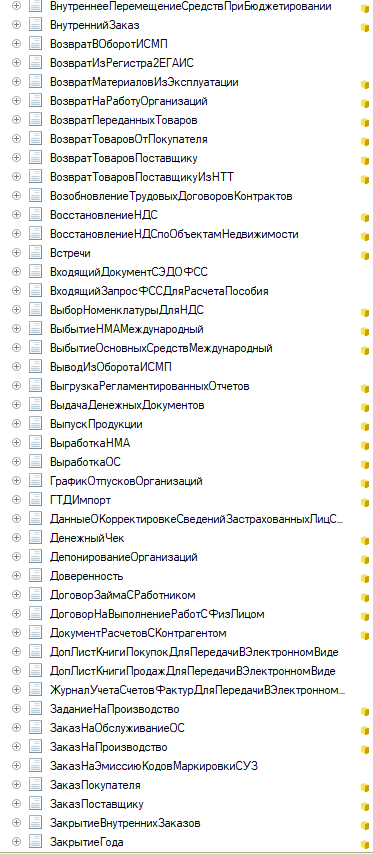
\includegraphics[width=0.5\linewidth]{images/documents}
	\caption{Пример отображения компонента Документы}
	\label{fig:documents}
\end{figure}

\paragraph{Справочники}

Компонент "Справочники" в 1С представляет собой один из основных инструментов для организации и хранения данных о различных объектах или сущностях, которые используются в программе. Он является одним из ключевых элементов в построении информационной модели прикладной системы и обеспечивает удобный и эффективный способ хранения, поиска и обработки данных.

На рисунке \ref{fig:spravochniki} представлен пример отображения компонента Справочники:
\begin{figure}
	\centering
	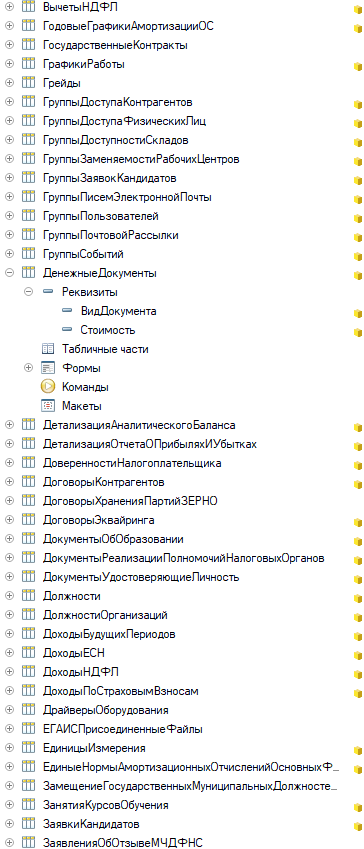
\includegraphics[width=0.5\linewidth]{images/spravochniki}
	\caption{Пример отображения компонента Справочники}
	\label{fig:spravochniki}
\end{figure}

\paragraph{Отчёты}

Компонент "Отчёты" в 1C предназначен для создания, настройки и запуска отчётов в рамках программной системы. Этот компонент имеет ключевое значение для аналитической работы и мониторинга различных аспектов бизнеса.

На рисунке \ref{fig:otchets} представлен пример отображения компонента Отчёты:

\begin{figure}
	\centering
	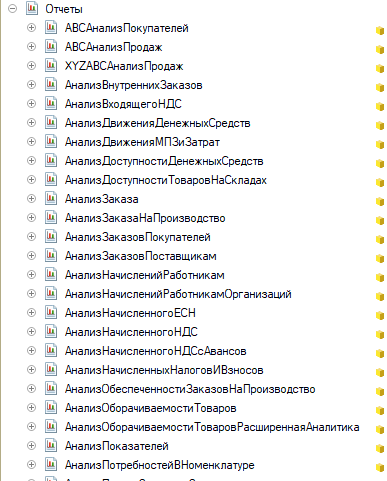
\includegraphics[width=0.5\linewidth]{images/otchets}
	\caption{Пример отображения компонента Отчёты}
	\label{fig:otchets}
\end{figure}

\paragraph{Регистры Сведений}

Компонент "Регистры сведений" в 1С предназначен для хранения и агрегации больших объёмов данных, которые не связаны напрямую с конкретными объектами (например, клиентами, заказами, товарами), но имеют важное значение для анализа и отчётности в системе.

На рисунке \ref{fig:registr1} представлен пример отображения компонента Регистры Сведений:
\begin{figure}
	\centering
	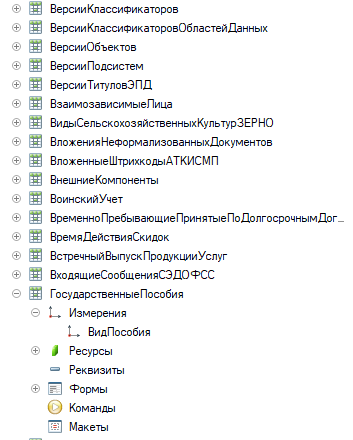
\includegraphics[width=0.5\linewidth]{images/registr1}
	\caption{Пример отображения компонента Регистры сведений}
	\label{fig:registr1}
\end{figure}

\paragraph{Константы}

Компонент "Константы" в 1C используется для хранения и управления постоянными значениями, которые используются в различных объектах конфигурации. Это могут быть, например, настройки, параметры или значения, которые редко изменяются и должны быть доступны из разных частей системы.

На рисунке \ref{fig:const1} представлен пример отображения компонента Константы:
\begin{figure}
	\centering
	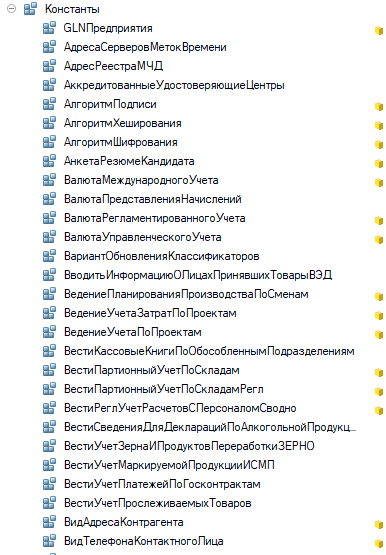
\includegraphics[width=0.5\linewidth]{images/const}
	\caption{Пример отображения компонента Константы}
	\label{fig:const}
\end{figure}